\documentclass[11pt,a4paper]{article}
\usepackage[margin=2.1cm,top=2.5cm,headheight=26pt]{geometry}
\usepackage{amsmath,amssymb,bm}
\usepackage{siunitx}
\usepackage{booktabs}
\usepackage{graphicx}
\usepackage{tikz}
\usetikzlibrary{arrows.meta,calc,positioning}
\usepackage{pgfplots}
\pgfplotsset{compat=1.17}
\usepackage{enumitem}
\usepackage{float}
\usepackage{xcolor}
\usepackage{pifont}
\newcommand{\cmark}{\textcolor{green!45!black}{\ding{51}}}
\newcommand{\xmark}{\textcolor{red!70!black}{\ding{55}}}
\usepackage{fancyhdr}
\usepackage{tcolorbox}
\tcbuselibrary{skins,breakable}
\usepackage[colorlinks=true,linkcolor=blue!60!black,urlcolor=blue!60!black]{hyperref}
\sisetup{per-mode=symbol,detect-all}
\graphicspath{{figs/}}

\definecolor{navy}{RGB}{25,53,73}
\newtcolorbox{keybox}[1]{title={#1},colback=blue!4,colframe=blue!50!black,fonttitle=\bfseries,breakable}
\newtcolorbox{aerobox}[1]{title={#1},colback=orange!5,colframe=orange!60!black,fonttitle=\bfseries,breakable}
\newtcolorbox{sumbox}[1]{title={#1},colback=green!4,colframe=green!40!black,fonttitle=\bfseries,breakable}

% Photograph slot: renders the image if present in figs/, else a dashed placeholder.
\newcommand{\photo}[4]{%
  \begin{figure}[H]\centering
  \IfFileExists{figs/#1.jpg}{\includegraphics[width=#2\linewidth]{#1}}{%
  \IfFileExists{figs/#1.png}{\includegraphics[width=#2\linewidth]{#1}}{%
    \begin{tikzpicture}
      \draw[dashed,gray,line width=0.8pt] (0,0) rectangle (#2\linewidth,0.52*#2\linewidth);
      \node[align=center,text width=0.82*#2\linewidth,font=\footnotesize\itshape,gray!70!black]
        at (0.5*#2\linewidth,0.26*#2\linewidth) {PHOTOGRAPH: #4\\[3pt]\ttfamily figs/#1.jpg};
    \end{tikzpicture}}}
  \caption{#3}
  \end{figure}}

\pagestyle{fancy}
\fancyhf{}
\lhead{
\includegraphics[height=0.6cm]{logos/itu_logo_laci.pdf}\ \ UCK 364E Design of Machine Elements}
\rhead{Case Study 4 --- Handout}
\lfoot{\footnotesize Department of Aeronautical Engineering, Istanbul Technical University}
\rfoot{\footnotesize Page \thepage}

\begin{document}

\begin{center}
{\Large\textbf{Case Study: Alaska Airlines Flight 261}}\\[3pt]
{\large\textbf{A wear point without an inspection is a scheduled failure}}\\[5pt]
{\small Prof.\ Dr.\ Onur Tunçer \ $\cdot$\ UCK 364E Design of Machine Elements}
\end{center}

\vspace{2pt}\hrule\vspace{6pt}

\noindent\emph{Why you are reading this.} Lecture 5 ended with a rule: if you make one element the
deliberate wear point of a mechanism, you incur three obligations --- specify the lubrication that
sets the wear rate, specify an inspection that measures the wear directly at an interval derived
from that rate, and either provide a second load path or state that there is none. This case study
is what happens when a competent organisation discharges none of the three. Every number in it
comes from a published investigation, and every one of them was available before the accident.

\section{What happened}

On \textbf{31 January 2000}, an Alaska Airlines McDonnell Douglas MD-83, registration N963AS,
operating flight 261 from Puerto Vallarta to San Francisco, suffered a jammed horizontal stabiliser
followed by a complete loss of pitch control. The aircraft entered an uncontrolled dive and struck
the Pacific Ocean off the California coast. All 88 people on board were killed.

\medskip
The component that failed is the one Lecture 5 ended on: the \textbf{horizontal stabiliser trim
jackscrew assembly}.

\photo{n963as}{0.68}{N963AS, the McDonnell Douglas MD-83 involved.}{N963AS in Alaska
Airlines livery}

\photo{flightpath}{0.84}{The track, with cockpit voice recorder timings. The first uncommanded
nose-down movement came at 16:09:20; the final dive began at 16:19:37. \textbf{The crew flew the
aircraft for ten minutes in between} --- long enough to diagnose it (``we have a jammed stabilizer
and we're maintaining altitude with difficulty''), long enough to plan, and not long enough for any
of it to matter, because there was nothing left to hold the stabiliser.}{NTSB flight track with CVR
callouts}

\photo{altitude}{0.58}{Preliminary altitude data from the Los Angeles airport surveillance radar.
The step at the left is the first event; the line at the right is the final descent from
\SI{18000}{ft}.}{NTSB preliminary altitude plot}

\section{The mechanism, and where the load goes}

\begin{figure}[H]\centering
\resizebox{0.66\textwidth}{!}{% The MD-80 horizontal stabiliser trim jackscrew, and where the load path runs.
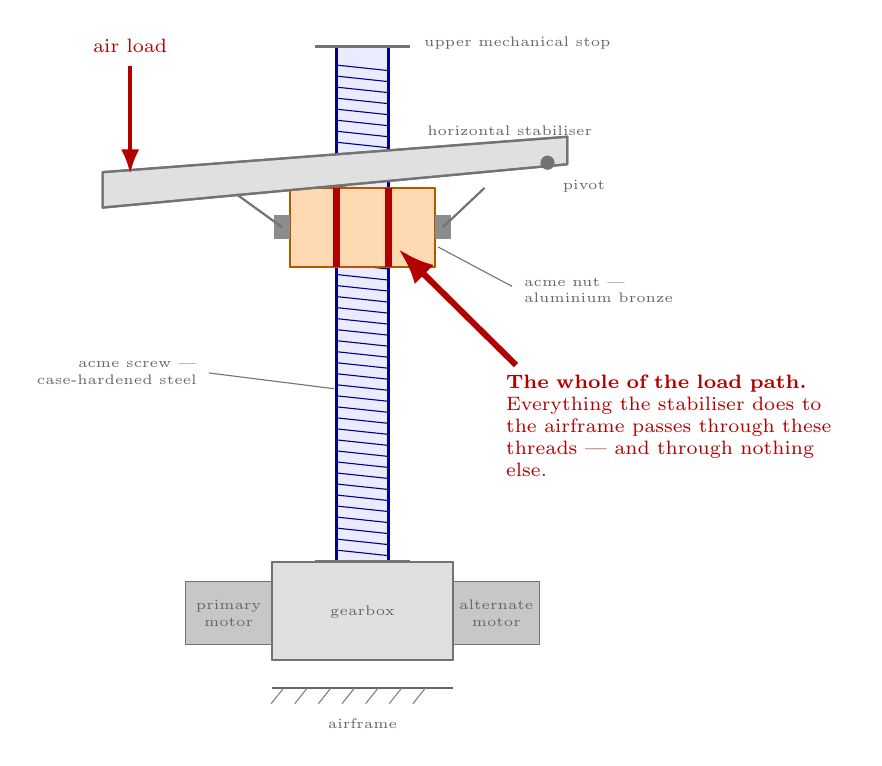
\begin{tikzpicture}[>=Latex,line join=round]
\tikzset{
  steel/.style={fill=blue!8,draw=blue!55!black,thick},
  brz/.style={fill=orange!30,draw=orange!70!black,thick},
  str/.style={fill=black!12,draw=black!55,thick},
  air/.style={->,red!70!black,line width=1.3pt},
  path/.style={red!70!black,line width=2.2pt},
  nt/.style={font=\scriptsize,align=left,text width=4.3cm},
  sm/.style={font=\tiny,text=black!60}
}

% ---------- the screw ----------
\draw[steel] (-0.33,0.55) rectangle (0.33,7.10);
\foreach \k in {0,1,...,44}{
  \pgfmathsetmacro\yy{0.70+0.14*\k}
  \ifdim\yy pt<7.05pt \draw[blue!55!black,thin] (-0.33,\yy) -- (0.33,\yy-0.07);\fi}
\draw[black!55,thin] (-1.95,2.95) -- (-0.36,2.75);
\node[sm,anchor=east,align=right] at (-1.98,2.95) {acme screw ---\\ case-hardened steel};

% ---------- the acme nut (gimbal nut) ----------
\fill[brz] (-0.92,4.30) rectangle (0.92,5.30);
\draw[orange!70!black,thick] (-0.92,4.30) rectangle (0.92,5.30);
\draw[path] (-0.33,4.30) -- (-0.33,5.30);
\draw[path] (0.33,4.30) -- (0.33,5.30);
\draw[black!55,thin] (1.90,4.05) -- (0.96,4.55);
\node[sm,anchor=west,align=left] at (1.93,4.00) {acme nut ---\\ aluminium bronze};

% gimbal pins out to the stabiliser
\fill[black!45] (-1.12,4.65) rectangle (-0.92,4.95);
\fill[black!45] (0.92,4.65) rectangle (1.12,4.95);

% ---------- the stabiliser ----------
\fill[str] (-3.30,5.05) -- (2.60,5.60) -- (2.60,5.95) -- (-3.30,5.50) -- cycle;
\draw[black!55,thick] (-3.30,5.05) -- (2.60,5.60) -- (2.60,5.95) -- (-3.30,5.50) -- cycle;
\node[sm,anchor=south west] at (0.70,5.84) {horizontal stabiliser};
\draw[black!55,thick] (-1.02,4.80) -- (-1.60,5.22);
\draw[black!55,thick] (1.02,4.80) -- (1.55,5.30);
\fill[black!55] (2.35,5.62) circle (0.09);
\node[sm,anchor=north west] at (2.42,5.52) {pivot};

% air load
\draw[air] (-2.95,6.85) -- (-2.95,5.48);
\node[font=\scriptsize,text=red!70!black,anchor=south] at (-2.95,6.90) {air load};

% ---------- stops ----------
\draw[black!55,very thick] (-0.60,7.10) -- (0.60,7.10);
\node[sm,anchor=west] at (0.66,7.14) {upper mechanical stop};
\draw[black!55,very thick] (-0.60,0.55) -- (0.60,0.55);

% ---------- gearbox and motors ----------
\fill[str] (-1.15,-0.70) rectangle (1.15,0.55);
\draw[black!55,thick] (-1.15,-0.70) rectangle (1.15,0.55);
\node[sm] at (0,-0.08) {gearbox};
\fill[black!22,draw=black!55] (-2.25,-0.50) rectangle (-1.15,0.30);
\fill[black!22,draw=black!55] (1.15,-0.50) rectangle (2.25,0.30);
\node[sm,align=center] at (-1.70,-0.10) {primary\\ motor};
\node[sm,align=center] at (1.70,-0.10) {alternate\\ motor};
\draw[black!60,thick] (-1.15,-1.05) -- (1.15,-1.05);
\foreach \k in {-1.0,-0.7,...,1.1}{\draw[black!50,thin] (\k,-1.05) -- (\k-0.16,-1.25);}
\node[sm,anchor=north] at (0,-1.32) {airframe};

% ---------- the load path annotation ----------
\draw[path,->] (1.95,3.05) -- (0.46,4.52);
\node[nt,anchor=north west,text=red!70!black] at (1.70,3.05)
 {\textbf{The whole of the load path.}\\ Everything the stabiliser does to the airframe passes
  through these threads --- and through nothing else.};

\end{tikzpicture}
}
\caption{The jackscrew assembly. The whole stabiliser pivots; the jackscrew holds its leading edge
against the air load for the entire flight.}
\label{fig:jack}
\end{figure}

The horizontal stabiliser is trimmed by pivoting the entire surface. A single Acme screw, driven by
a primary and an alternate motor through a gearbox, turns inside an Acme nut; the nut is gimballed
to the stabiliser. Turn the screw and the nut travels, and the stabiliser rotates about its pivot.

\medskip
Three facts about this arrangement matter, and all three are Lecture 5 material.

\begin{enumerate}[leftmargin=*,itemsep=2pt]
\item \textbf{It is self-locking.} An Acme thread at this lead angle will not back-drive, which is
  exactly why it can hold the stabiliser against air load with both motors switched off. The
  self-locking that makes it a good trim actuator is the same property that makes the nut thread
  the only thing resisting the load.
\item \textbf{It is a single load path.} Everything the stabiliser does to the airframe passes
  through the engagement between the nut threads and the screw threads. There is nothing else.
\item \textbf{The nut is the designed wear point.} The screw threads are \emph{case-hardened steel};
  the nut threads are \emph{aluminium bronze}, about \SI{0.15}{in} thick at the minor diameter when
  new. The soft component is deliberately sacrificial: it is cheaper to replace a nut than a screw,
  and the wear is concentrated where you can predict and inspect it.
\end{enumerate}

\photo{finaccess}{0.56}{The assembly is reached through the leading edge of the vertical fin, from
a man-lift. The end play check on which the whole safety case rested is a scheduled, awkward,
easily deferred job --- which is part of why extending its interval is always tempting.}{jackscrew
access panel in the fin, with maintenance stand}

\medskip
Point 3 is a good design decision. It is the decision Lecture 5 says you are allowed to make ---
\emph{provided} you then do the three things it obliges you to do.

\section{The two numbers that were supposed to keep it safe}

\subsection*{Lubrication --- which sets the wear rate}

The original Douglas process standard, at DC-9 certification in 1964, called for the jackscrew to be
lubricated every \textbf{300 to 350 flight hours}. Later maintenance documents extended this; Alaska
Airlines lubricated at every other B check from 1985 --- about every \textbf{700 flight hours} ---
and subsequent revisions lengthened it further.

\subsection*{The end play check --- which measures the wear directly}

As the loaded flank of the nut thread wears away, the nut can move axially along the screw before
the flanks make contact. That lost motion is \textbf{end play}, and it is read off a dial gauge on
the assembled mechanism without taking anything apart. It is a direct measurement of the damage ---
precisely the kind of inspection Lecture 5 asks for.

\medskip
The rule was simple: \textbf{the Acme nut was to be replaced when the end play measurement exceeded
\SI{0.040}{in}.}

\begin{keybox}{The limit is not a strength limit --- and this is the whole point}
Boeing's testimony to the investigation gives two numbers that students usually find surprising:

\begin{center}\small
\begin{tabular}{@{}p{5.0cm}p{9.4cm}@{}}
\toprule
A \textbf{new} Acme nut & ``the strength of the threads is over \textbf{15 times} in excess of
  design loads''\\[2pt]
Worn to the \SI{0.040}{in} \textbf{replacement limit} & ``remains \textbf{10 times} stronger'' than
  the maximum design loads\\
\bottomrule
\end{tabular}
\end{center}

\medskip
So the replacement limit is not the point at which the thread becomes weak. At the limit the part
still has a margin most structures would envy. The limit exists for one reason only: \textbf{to tell
you the wear rate while there is still margin left to act on}. Its entire value is \emph{information},
and information has a shelf life. A limit you do not measure often enough is not a limit at all.
\end{keybox}

\section{The arithmetic, in the symbols of Lecture 5}

\subsection{The wear is not linear --- and the design assumed it was}

Among the safety assumptions the investigation identified behind this design was that
\emph{``the wear rate of the Acme nut thread was linear.''} Lecture 5, Example 5.2, says otherwise.

\medskip
The thread carries the load on its flank. The bearing area falls in proportion to the remaining
thickness $t$, so the bearing pressure rises as
\[
p \;\propto\; \frac{1}{t}.
\]
Take the simplest wear law consistent with that --- wear rate proportional to pressure, as in
Archard's relation. Then
\[
\frac{\mathrm{d}x}{\mathrm{d}N}\;\propto\;p\;\propto\;\frac{1}{t},
\qquad t = t_0 - x
\qquad\Longrightarrow\qquad
t\,\mathrm{d}t \propto -\,\mathrm{d}N
\qquad\Longrightarrow\qquad
\boxed{\;t^{2}\ \text{falls linearly with }N\;}
\]
so that $t = t_0\sqrt{1 - N/N_f}$. The consequence is the one that matters:

\begin{center}\small
\begin{tabular}{@{}lccc@{}}
\toprule
 & wear depth $x$ & \% of the \emph{depth} & \% of the \emph{life}\\
\midrule
New & \SI{0}{in} & 0 & 0\\
At the \SI{0.040}{in} replacement limit & \SI{0.037}{in} & 26 & \textbf{43}\\
Contact retreats to the root & \SI{0.080}{in} & 57 & 78\\
Thread shears & \SI{0.140}{in} & 100 & 100\\
\bottomrule
\end{tabular}
\end{center}

\medskip
Read the last two columns against each other. At the replacement limit you have consumed about a
quarter of the material but \textbf{nearly half of the life}. A maintenance programme that treats
wear as linear will therefore always over-estimate how long it has left --- and will do so by more
and more as the part gets closer to failure.

\begin{figure}[H]\centering
\resizebox{\textwidth}{!}{% One acme nut thread in axial section, at four stages of wear. Screw axis horizontal.
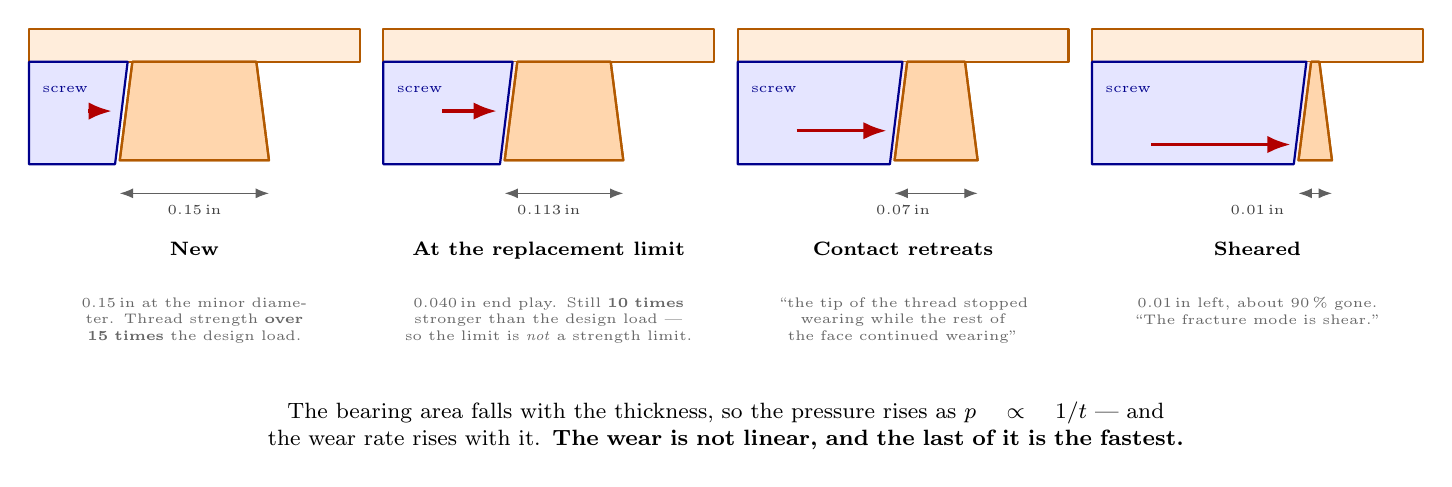
\begin{tikzpicture}[>=Latex,line join=round]
\tikzset{
  brz/.style={fill=orange!32,draw=orange!70!black,thick},
  body/.style={fill=orange!14,draw=orange!70!black,thick},
  gone/.style={fill=red!7,draw=red!50,thin,dashed},
  scr/.style={fill=blue!10,draw=blue!55!black,thick},
  ld/.style={->,red!70!black,line width=1.2pt},
  ttl/.style={font=\scriptsize\bfseries,align=center,text width=4.0cm,anchor=north},
  sub/.style={font=\tiny,align=center,text width=3.7cm,text=black!60,anchor=north}
}
\def\S{10.5}      % in -> cm, thickness scale
\def\Ht{1.25}     % tooth height (radial)
\def\tap{0.16}    % half-taper

% \tooth{x centre}{wear depth, in}{contact height fraction}{title}{subtitle}
\newcommand{\tooth}[5]{%
  \pgfmathsetmacro\tn{0.15*\S}            % new half-widths
  \pgfmathsetmacro\tw{(0.15-#2)*\S}       % worn thickness
  \pgfmathsetmacro\w{#2*\S}               % material lost, off the left flank
  % nut body above, bore to left and right
  \fill[body] (#1-2.10,\Ht) rectangle (#1+2.10,\Ht+0.42);
  % ghost of the original tooth
  \ifdim #2pt>0pt
    \fill[gone] (#1-\tn/2-\tap,0) -- (#1+\tn/2+\tap,0)
             -- (#1+\tn/2,\Ht) -- (#1-\tn/2,\Ht) -- cycle;
  \fi
  % the remaining tooth: left flank has retreated by \w
  \fill[brz] (#1-\tn/2-\tap+\w,0) -- (#1+\tn/2+\tap,0)
          -- (#1+\tn/2,\Ht) -- (#1-\tn/2+\w,\Ht) -- cycle;
  \draw[orange!70!black,thick] (#1-\tn/2-\tap+\w,0) -- (#1+\tn/2+\tap,0)
          -- (#1+\tn/2,\Ht) -- (#1-\tn/2+\w,\Ht) -- cycle;
  % the screw flank bearing on it, pushing left-to-right
  \fill[scr] (#1-2.10,-0.05) -- (#1-\tn/2-\tap+\w-0.06,-0.05)
          -- (#1-\tn/2+\w-0.06,\Ht) -- (#1-2.10,\Ht) -- cycle;
  \node[font=\tiny,text=blue!55!black,anchor=west] at (#1-2.05,\Ht*0.72) {screw};
  % load, applied over the part of the flank still in contact
  \pgfmathsetmacro\yc{\Ht*#3}
  \draw[ld] (#1-1.35,\yc) -- (#1-\tn/2-\tap+\w-0.10,\yc);
  % thickness at the tip (minor diameter), where the 0.15 in is quoted
  \draw[<->,gray!75!black,thin] (#1-\tn/2-\tap+\w,-0.42) -- (#1+\tn/2+\tap,-0.42);
  \node[font=\tiny,anchor=north,text=gray!50!black] at (#1,-0.44)
    {\pgfmathparse{0.15-#2}\pgfmathprintnumber[fixed,precision=3]{\pgfmathresult}\,in};
  \node[ttl] at (#1,-0.92) {#4};
  \node[sub] at (#1,-1.62) {#5};
}

\tooth{0}{0.000}{0.50}{New}{\SI{0.15}{in} at the minor diameter. Thread strength \textbf{over 15 times} the design load.}
\tooth{4.5}{0.037}{0.50}{At the replacement limit}{\SI{0.040}{in} end play. Still \textbf{10 times} stronger than the design load --- so the limit is \emph{not} a strength limit.}
\tooth{9.0}{0.080}{0.30}{Contact retreats}{``the tip of the thread stopped wearing while the rest of the face continued wearing''}
\tooth{13.5}{0.140}{0.16}{Sheared}{\SI{0.01}{in} left, about \SI{90}{\percent} gone. ``The fracture mode is shear.''}

\node[font=\footnotesize,align=center,text width=15.5cm,anchor=north] at (6.75,-2.95)
 {The bearing area falls with the thickness, so the pressure rises as $p\propto1/t$ --- and the wear
  rate rises with it. \textbf{The wear is not linear, and the last of it is the fastest.}};

\end{tikzpicture}
}
\caption{One Acme nut thread in axial section. The loaded flank retreats; the contact patch moves
down toward the root; the pressure on what remains rises throughout.}
\label{fig:wear}
\end{figure}

\subsection{What the inspection interval actually bought}

On \textbf{30 September 1997}, during a C check at Oakland, the end play on N963AS was measured.
The first reading was \textbf{\SI{0.040}{in}} --- at the limit --- and the nut was ordered replaced.
The check was then re-taken, recorded as \emph{``Found end play to be within limits .033 \dots\
Rechecked five times with same result,''} and the nut was \textbf{not} replaced.

\medskip
Boeing's own conversion between end play and thread loss is that \SI{0.040}{in} of end play
corresponds to roughly \SIrange{0.030}{0.037}{in} of thread thickness gone. Scaling, the accepted
\SI{0.033}{in} reading implies about \SIrange{0.025}{0.031}{in} already lost --- call it
\SI{0.12}{in} of the original \SI{0.15}{in} still there.

\medskip
That was the \emph{last} end play check carried out on the aircraft. In the
\textbf{28 months and nearly 9\,000 flight hours} that followed, no further end play check fell due.

\begin{figure}[H]\centering
\resizebox{\textwidth}{!}{% Nut thread wear against flight hours, with the inspection opportunities that existed.
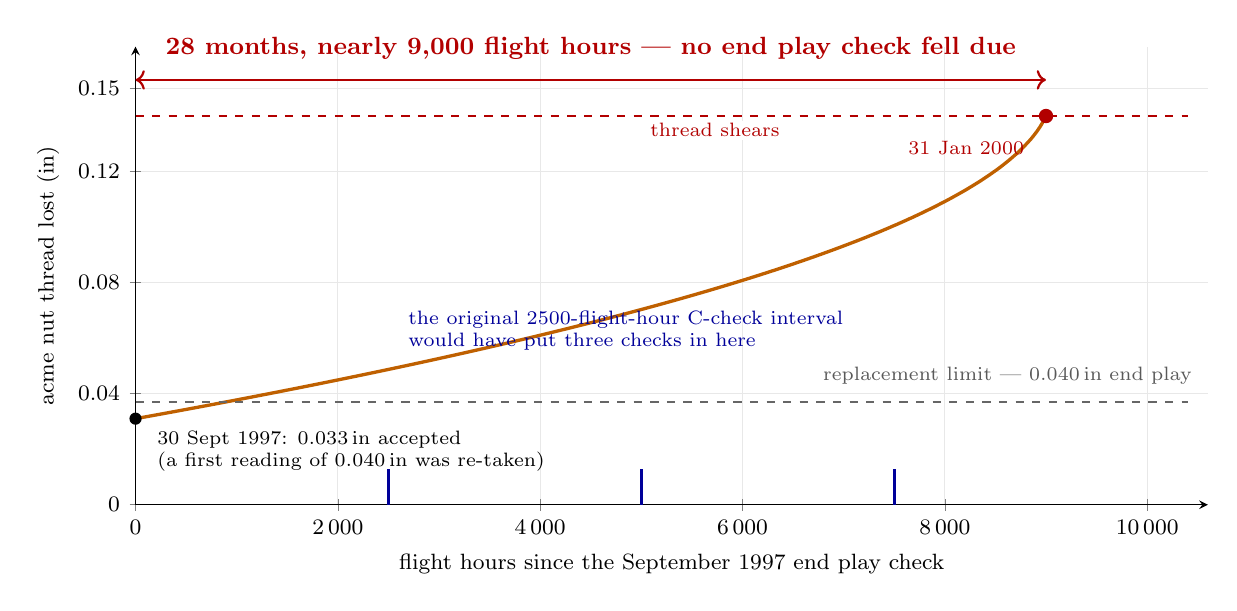
\begin{tikzpicture}
\begin{axis}[
  width=15.2cm,height=7.4cm,
  xlabel={flight hours since the September 1997 end play check},
  ylabel={acme nut thread lost (in)},
  xmin=0,xmax=10600,ymin=0,ymax=0.165,
  xtick={0,2000,4000,6000,8000,10000},
  scaled x ticks=false,
  xticklabel style={/pgf/number format/fixed,/pgf/number format/1000 sep={\,}},
  ytick={0,0.04,0.08,0.12,0.15},
  yticklabel style={/pgf/number format/fixed,/pgf/number format/precision=2},
  label style={font=\footnotesize},tick label style={font=\footnotesize},
  grid=both,grid style={gray!18},
  axis lines=left,clip=false]

% ---- the wear curve: Archard with p ~ 1/t gives t^2 linear in N ----
% starts at 0.031 in already lost, reaches 0.140 in at 9000 FH
\addplot[very thick,orange!75!black,domain=0:9000,samples=300]
  {0.15 - sqrt( (0.15-0.031)^2 - ((0.15-0.031)^2-(0.15-0.140)^2)*x/9000 )};

% ---- the two levels that matter ----
\draw[dashed,black!60] (axis cs:0,0.037) -- (axis cs:10400,0.037);
\node[font=\scriptsize,anchor=south west,text=black!65] at (axis cs:6700,0.040)
  {replacement limit --- \SI{0.040}{in} end play};
\draw[dashed,red!70!black,thick] (axis cs:0,0.140) -- (axis cs:10400,0.140);
\node[font=\scriptsize,anchor=north east,text=red!70!black,fill=white,inner sep=1pt]
  at (axis cs:6400,0.1385) {thread shears};

% ---- where it started ----
\fill[black] (axis cs:0,0.031) circle (2.2pt);
\node[font=\scriptsize,anchor=north west,align=left] at (axis cs:120,0.030)
  {30 Sept 1997: \SI{0.033}{in} accepted\\ \scriptsize(a first reading of \SI{0.040}{in} was re-taken)};

% ---- the accident ----
\fill[red!70!black] (axis cs:9000,0.140) circle (2.6pt);
\node[font=\scriptsize,anchor=north east,text=red!70!black,align=right]
  at (axis cs:8880,0.1345) {31 Jan 2000};

% ---- the span with no end play check due ----
\draw[<->,red!70!black,thick] (axis cs:0,0.153) -- (axis cs:9000,0.153);
\node[font=\small\bfseries,text=red!70!black,anchor=south]
  at (axis cs:4500,0.157) {28 months, nearly 9{,}000 flight hours --- no end play check fell due};

% ---- what the original interval would have given ----
\draw[blue!60!black,very thick] (axis cs:2500,0) -- (axis cs:2500,0.013);
\draw[blue!60!black,very thick] (axis cs:5000,0) -- (axis cs:5000,0.013);
\draw[blue!60!black,very thick] (axis cs:7500,0) -- (axis cs:7500,0.013);
\node[font=\scriptsize,text=blue!60!black,anchor=south west,align=left]
  at (axis cs:2600,0.052)
  {the original \mbox{2500-flight-hour} C-check interval\\ would have put three checks in here};

\end{axis}
\end{tikzpicture}
}
\caption{The wear that had to occur between the last measurement and the accident, on the
$t^{2}$ law above. Whatever the interval said on paper, the observed fact is that no opportunity to
measure fell inside it.}
\label{fig:interval}
\end{figure}

\begin{keybox}{The damage-tolerance arithmetic, done the way Lecture 4 does it}
Over that span the nut lost roughly $0.140-0.031 = \SI{0.11}{in}$ of thread in \num{9000} flight
hours, an average of about
\[
\SI{0.012}{in\ per\ 1000\ flight\ hours}.
\]
At that rate, the window between the \emph{replacement limit} and \emph{failure} is
\[
N_{\text{window}} = \frac{0.140-0.037}{0.012}\times 1000 \approx \SI{8500}{flight\ hours}.
\]
Lecture 4's rule for any inspection-based safety argument is that the interval must divide the
window at least twice: $n = N_{\text{window}}/\text{interval} \ge 2$.

\begin{center}\small
\begin{tabular}{@{}lcc@{}}
\toprule
End play check at\dots & interval & $n$\\
\midrule
the original \num{2500}-flight-hour C check & \SI{2500}{FH} & \textbf{3.4} \ \cmark\\
a 15-month C check & $\approx\SI{4775}{FH}$ & 1.8 \ --- already marginal\\
what actually elapsed, with none due & \SI{9000}{FH} & \textbf{0.9} \ \xmark\\
\bottomrule
\end{tabular}
\end{center}

\medskip
\textbf{The safety case did not degrade. It went to zero.} With fewer than one opportunity in the
window, the inspection could not detect the wear before failure \emph{even if it had been performed
perfectly}. And it would not have been performed perfectly: Alaska's end play restraining fixture
was made in-house and was not the manufacturer's tool. The airline itself later told the FAA that
\emph{``some of these tools could bottom out during the check, thus potentially yielding an
erroneous measurement.''}
\end{keybox}

\subsection{And the lubrication never reached the threads}

When the assembly was recovered, the investigators found no grease where grease does the work:
\emph{``There was no visible evidence of grease on the acme screw along the length where it normally
travels''}, and \emph{``There was no visible evidence of grease on the inner diameter of the acme
nut.''} Globules of fresh grease were found on the \emph{outside} of the assembly. The FAA's account
records that the grease fitting passage that feeds the threads was found plugged with dry residue,
so that the assembly was ``essentially unlubricated''.

\medskip
This is the first obligation failing in the most ordinary way possible. The lubrication was
scheduled. Someone signed for it. It went onto the outside of a fitting whose passage was blocked,
and the number that the whole wear calculation depended on --- the coefficient of friction between
bronze and steel --- quietly became a different number.

\section{What was found, and what the investigation concluded}

The recovered nut had \emph{``only small ridges of the acme thread remaining''}; elsewhere the
examination records \emph{``no threads''} on the inner diameter, with helical marks along its whole
length. Approximately \textbf{90\,\%} of the thread thickness had worn away before the remainder
sheared. The sheared material was found as \emph{``several flat ribbons of metal, resembling an acme
nut thread remnant \dots\ coiled in the valleys''} of the screw --- bronze in colour, about
\SI{0.025}{in} thick. The thread had not only failed; its remains had wrapped themselves around the
screw and jammed it.

\photo{recovery}{0.62}{Wreckage being landed during the recovery operation. The jackscrew assembly
was recovered from the sea floor and became the central physical evidence of the investigation.}{night recovery
of wreckage on a dock}

\photo{jackscrew}{0.30}{The recovered Acme screw. The bronze ribbons coiled in the thread valleys
are the remains of the nut thread that should have been carrying the stabiliser.}{the recovered
jackscrew with thread remnants wrapped around it}

\begin{aerobox}{The probable cause, in full}
\emph{``A loss of airplane pitch control resulting from the in-flight failure of the horizontal
stabilizer trim system jackscrew assembly's acme nut threads. The thread failure was caused by
excessive wear resulting from Alaska Airlines' insufficient lubrication of the jackscrew assembly.}

\medskip
\emph{Contributing to the accident were Alaska Airlines' extended lubrication interval and the
Federal Aviation Administration's (FAA) approval of that extension, which increased the likelihood
that a missed or inadequate lubrication would result in excessive wear of the acme nut threads, and
Alaska Airlines' extended end play check interval and the FAA's approval of that extension, which
allowed the excessive wear of the acme nut threads to progress to failure without the opportunity
for detection. Also contributing to the accident was the absence on the McDonnell Douglas MD-80 of a
fail-safe mechanism to prevent the catastrophic effects of total acme nut thread loss.''}

\medskip
\hfill --- NTSB/AAR-02/01, adopted 10 December 2002
\end{aerobox}

\medskip
On the third element, the investigation was explicit that the design did not account for the loss of
the Acme nut threads as a catastrophic single-point failure mode, and that \emph{``the dual-thread
design of the Acme screw nut does not provide redundancy with respect to wear''} --- both thread
sets were load-bearing, so wear that consumed one consumed the other.

\section{The three obligations, checked}

Lecture 5 stated the rule before you knew this case existed. Hold the accident against it.

\begin{center}\small
\begin{tabular}{@{}p{6.1cm}p{10.0cm}@{}}
\toprule
The obligation & What happened\\
\midrule
\textbf{1.} Specify the lubrication that sets the wear rate you assumed. &
  Interval extended from \numrange{300}{350} flight hours to \num{700} and beyond --- and the
  grease never reached the threads at all. The assumed wear rate was therefore never the actual
  one.\\[3pt]
\textbf{2.} Specify an inspection that measures the wear \emph{directly}, at an interval derived
  from that rate \emph{with the acceleration included}. &
  The right inspection existed and measured the right quantity. Its interval was extended until it
  gave \textbf{fewer than one} opportunity inside the window --- and the rate it was derived from
  was assumed linear, when the physics says $t^2$.\\[3pt]
\textbf{3.} Provide a second load path, or state explicitly that there is none and that the
  inspection is therefore the whole of the safety case. &
  There was no second load path, and the design did not treat total thread loss as a credible
  failure mode. The inspection \emph{was} the whole safety case --- which is exactly why item 2
  was fatal.\\
\bottomrule
\end{tabular}
\end{center}

\begin{sumbox}{What this case is actually about}
Not lubrication. Not one airline. The failure is a \textbf{reasoning} failure, and it is one you
can commit in an afternoon with a spreadsheet:

\medskip
\textbf{Each interval extension was defensible on its own.} Nothing had broken. The fleet data
looked fine. What nobody re-derived was the quantity that actually mattered --- the number of
opportunities to detect the wear before it became failure. That number is
$n = N_{\text{window}}/\text{interval}$, and it had fallen below one while every individual decision
still looked reasonable.

\medskip
A damage-tolerance argument is not a schedule. It is an \emph{inequality}, and it has to be
re-checked every single time you change either side of it.
\end{sumbox}

\section{What changed because of it}

The investigation produced recommendations on lubrication procedure and intervals, on end play check
procedure and tooling standardisation, and on the treatment of wear as a failure mode in
certification. More broadly, this accident --- together with the fuselage and structural cases you
have already met --- is why ``the inspection will catch it'' is no longer accepted as a safety
argument unless the interval is derived from a measured growth rate and demonstrated to divide the
window at least twice.

\section{Questions to think about}

\begin{enumerate}[leftmargin=*,itemsep=3pt]
\item The \SI{0.040}{in} limit left a $10\times$ strength margin. Argue \emph{for} setting a
  replacement limit that conservative, then argue \emph{against} it. Which argument does this
  accident support, and why is that not the obvious answer?
\item Using the $t^2$ wear law, derive the interval that would have given $n=3$ from the
  \SI{0.033}{in} measurement. Compare it with the original \num{2500}-flight-hour C check. What does
  the comparison tell you about how the original interval was probably chosen?
\item The first reading was \SI{0.040}{in} and the second \SI{0.033}{in}. Suppose you are the
  engineer on shift. Write the two-sentence rule you would want in the manual governing what happens
  when a re-check disagrees with a first reading on a single-load-path component.
\item Propose a fail-safe for this mechanism. You may not add a second jackscrew. State what your
  device carries, what it does \emph{not} protect against, and how it is inspected --- because a
  fail-safe you cannot inspect has just become the new single point of failure.
\item The nut is the sacrificial element because it is softer. Suppose you reverse it and make the
  \emph{screw} sacrificial. List every consequence, and say whether the trade is worth making.
\end{enumerate}

\section*{Sources and image credits}

\begin{itemize}[leftmargin=*,itemsep=1pt,font=\footnotesize]
\item[] {\footnotesize National Transportation Safety Board, \emph{Loss of Control and Impact with
  Pacific Ocean, Alaska Airlines Flight 261, McDonnell Douglas MD-83, N963AS, About 2.7 Miles North
  of Anacapa Island, California, January 31, 2000}, NTSB/AAR-02/01.}
\item[] {\footnotesize NTSB public docket DCA00MA023 --- Group Chairman Factual Reports
  (Systems--Powerplants, Structures, Maintenance Records) and the Jackscrew Gimbal Nut Thread
  Remnant Formation Study. Source of the recovered-condition quotations and the September 1997 work
  card.}
\item[] {\footnotesize NTSB Safety Recommendations A-02-36 through -51.}
\item[] {\footnotesize FAA \emph{Lessons Learned from Transport Airplane Accidents}, N963AS. Source
  of the \SI{90}{\percent} thread-loss figure and the plugged grease fitting passage.}
\item[] {\footnotesize \emph{Images.} Flight track, altitude plot and recovered-jackscrew
  photographs are from the NTSB investigation of this accident. Remaining photographs are
  reproduced for teaching purposes only.}
\end{itemize}

\vspace{4pt}
\noindent{\footnotesize\emph{Note on the arithmetic.} The wear-rate, window and $n$ figures in
\S4 are worked in this handout from published measurements; they are not quoted from the
investigation, which did its own analysis by other means. They are here because they are the
calculation \emph{you} are being taught to do, and because they can be checked against the
published numbers line by line.}

\end{document}
